\documentclass[aspectratio=169]{beamer}
%\documentclass[aspectratio=43]{beamer}

\usepackage{graphicx}  % Required for including images
\usepackage{natbib}
\usepackage{booktabs} % Top and bottom rules for tables
\usepackage{amssymb,amsthm,amsmath}
\usepackage{exscale}
\usepackage{natbib}
\usepackage{tikz}
\usepackage{listings}
\usepackage{color}
\usepackage{bm}
% Setup TikZ
\usepackage{tikz}
\usetikzlibrary{arrows}
\tikzstyle{block}=[draw opacity=0.7,line width=1.4cm]
% Setup hyperref
\usepackage{hyperref}
\hypersetup{colorlinks=true}
\hypersetup{citecolor=porange}
\hypersetup{urlcolor=porange!80!}
\hypersetup{linkcolor=porange}

\newtheorem{proposition}{Proposition}
\newtheorem{remark}{Remark}
\newtheorem{principle}{Principle}

%% Writing quarters
\newcommand{\wQ}[1]{{\textcolor{white}{Q#1}}}
\newcommand{\bQ}[1]{{Q#1}}

% Uncomment appropriate command to disable/enable hiding
\newcommand{\mypause}{\pause}
%\newcommand{\mypause}{}
\newcommand{\myb}[1]{{\color{blue} {#1}}}

\DeclareMathAlphabet{\mathpzc}{OT1}{pzc}{m}{it}

%% Autoscaled figures
\newcommand{\incfig}{\centering\includegraphics}
\setkeys{Gin}{width=0.9\linewidth,keepaspectratio}

%Make the items smaller
\newcommand{\cramplist}{
	\setlength{\itemsep}{0in}
	\setlength{\partopsep}{0in}
	\setlength{\topsep}{0in}}
\newcommand{\cramp}{\setlength{\parskip}{.5\parskip}}
\newcommand{\zapspace}{\topsep=0pt\partopsep=0pt\itemsep=0pt\parskip=0pt}

\newcommand{\backupbegin}{
   \newcounter{finalframe}
   \setcounter{finalframe}{\value{framenumber}}
}
\newcommand{\backupend}{
   \setcounter{framenumber}{\value{finalframe}}
}

\usetheme[bullet=circle,% Use circles instead of squares for bullets.
          titleline=true,% Show a line below the frame title.
          ]{Princeton}

\title[{\tt }] {Lecture 14: Software and Hardware Issues in Computational Physics}%
\author[https://apc523-2020.rtfd.io]%
{Ammar H. Hakim ({\tt ahakim@pppl.gov}) \inst{1}}%

\institute[PPPL]
{ \inst{1} Princeton Plasma Physics Laboratory, Princeton, NJ %
}

\date[3/23/2020]{Princeton University, Course APC523, 2020}

\begin{document}

\begin{frame}[plain]
  \titlepage
\end{frame}

%----------------------------------------------------------------
\begin{frame}{Goal: Hardware and software for Computational Physics}
  Our computation physics codes must run somewhere: Making code work
  on modern hardware and writing \emph{long-lived} and \emph{usable}
  software is highly non-trivial task. {\bf Difficult
    and under appreciated art!}
  \begin{itemize}
  \item Modern computer hardware is changing: new architectures are
    emerging (too) rapidly.
    \begin{itemize}\cramplist
    \item Pressure on hardware: make chips \emph{faster} but
      \emph{consume less energy}. Contradictory goals.
    \item New directions: many (100s or 1000s) more low-power
      ``cores'' with lower clock speed.
    \end{itemize}
  \item Software is expensive, even (and especially) when it is free!
    \begin{itemize}\cramplist
    \item Software development is \emph{labor intensive}. Takes time,
      and humans get tired, need to sleep, eat, take vacations (and
      hide from viruses).
    \item More importantly: writing good code is an \emph{art}. Can't
      be learned only from books. Need to \emph{apprentice} yourself
      with a Master Craftsman. Process is slow, can take years to
      perfect art.
    \end{itemize}
  \end{itemize}
\end{frame}
% ----------------------------------------------------------------

% ----------------------------------------------------------------
\begin{frame}{How fast (in principle) is my Mac?}
  \footnotesize%
  Mid 2015, Intel Core i7 chip.  See
  \href{https://everymac.com/systems/apple/macbook_pro/specs/macbook-pro-core-i7-2.8-15-iris-only-mid-2015-retina-display-specs.html}{See
    this page} for info on chips which ship with different
  Macs. Strangely, this information is not in the ``About this Mac''
  tab and one needs to go digging for it.
  \begin{itemize}
  \item Clock-speed is $2.8$~GHz. So we have $2.8$~GFLOPS/core
    (assuming a FLOP can be done in 1 cycle).%
    \mypause%
  \item However, SIMD can potentially do 4 FLOPS per cycle (for {\tt
      float}. For {\tt double} SIMD is 2 FLOPS per cycle). Giving
    $11.2$~GFLOPS/core.%
    \mypause%
  \item Often there are are multiple FPUs (floating point units) on a
    core. Mine has 2 FPUs (AFAICT. The specs say total 8 ``threads''
    which I assume means 2 FPUs per-core), but some chips have 4
    FPUs. So that brings it to $22.4$~GFLOPS/core.
  \item With 4 cores this gives $89.6$~GFLOPS (half of that for {\tt
      double} precision numbers) total.
  \end{itemize}
  Our Eigen double matrix-matrix multiply peaked at about $8$~GFLOPS
  on a single core. Float matrix-matrix multiple peaked at about
  $15$~GFLOPS.%
  \mypause%
  \vskip0.1in%
  Eigen's peformance comes from ``tiling'' the matrix and using SIMD
  instructions. (Most PDE solvers can't always use such tricks. Linear
  algebra is very specialized. Best left to experts). 
\end{frame}
% ----------------------------------------------------------------

% ----------------------------------------------------------------
\begin{frame}{It is hard to achieve anything close to
    peak-performance}
  \begin{itemize}
  \item Memory access will slow down a program by a lot: FLOPS are not
    the only thing that matter!
  \item If you get between $10$-$20\%$ peak you are in (very) good
    shape. More likely, $5\%$ peak is reasonable.
  \item My team's code ({\tt Gkeyll}) gets 500~GFLOPS for some compute
    kernels on an Intel Skylake chip (peak-performance of
    3~TFLOPS). Does not use SIMD vectorization (due to our code
    structure SIMD is hard to use). This is pretty good.
  \item Similar performance is obtained on a Mac: 12~GFLOPS on a
    4-core Mac. (Skylake chips have 48 cores and are $3\times$
    faster).
  \end{itemize}
  {\bf Study Agner Fog's optimization manuals if you are serious about
    optimization}. PU PICSciE (Reasearch Computing) offers workshops.
\end{frame}
% ----------------------------------------------------------------

%----------------------------------------------------------------
\begin{frame}{Some (brief) notes on software engineering}
  \footnotesize%
  If you read only one book on Software Engineering, it
  should be the ``Mythical Man Month''.

  \begin{columns}
    \begin{column}{0.4\linewidth}
      
\includegraphics[width=0.8\linewidth]{mmm.pdf}
    \end{column}
    
    \begin{column}{0.6\linewidth}
      TL;DR Version: 
      \begin{itemize}
      \item Writing large-scale software programs is hard. 
      \item Techiques that work on small projects don't scale to large
        projects. It is important to learn by looking at good, large
        code bases.
      \item Most of physicists won't work on such projects, but these
        are now becoming increasingly important. Consider the SCIDAC
        program, which supports huge codes, running into 100K+ (even
        millions of) lines of code (LOC), with multiple developers,
        are massively parallel and are designed to solve very complex
        physical problems.
      \end{itemize}
    \end{column}
  \end{columns}
    
\end{frame}
%----------------------------------------------------------------

%----------------------------------------------------------------
\begin{frame}{Some (brief) notes on software engineering}
  \footnotesize%
  Large-scale computational physics software is, in some ways, even
  harder, as it is not clear if one is solving the equations correctly
  (\emph{verification}) and if one has the correct model in the first
  place (\emph{validation}). \emph{Regression testing} and careful
  benchmarks are essential to build confidence.
  % 
  \mypause%
  \vskip0.05in%
  Some general recommendations for ``small'' projects (thesis level)
  \begin{itemize}
  \item Unless you are working on an existing ``old'' code, use modern
    C++. It is hard to find libraries, and general support for
    high-level things in Fortran (scripting, flexible input files,
    ...). Hard to find jobs.%
    \mypause%
  \item Don't invent your own. There are a huge amount of existing
    math libraries (LAPACK/BLAS, GSL, PETSC, Eigen, Boost, FFTW,
    SuperLU, HDF5 ....), and it is unlikely you can write a better
    routine in a short amount of time.%
    \mypause%
  \item Use a version control system, \emph{even for small
      projects}. Git is a good option, and code can be hosted for free
    on github or bitbucket.%
    \mypause%
  \item Use an automated build system. \href{https://cmake.org}{CMake}
    has a lot of momentum, and is a very good choice. There are other
    possible choices too. I like \href{https://waf.io}{Waf} a lot.
  \end{itemize}
  \mypause%
  A reasonable stack: C++ and Eigen with CMake build system, with HDF5
  or NETCDF output format, GSL, PETSC, ..., and post-processing using
  Python (Anaconda Python is an excellent free distribution with
  everything you need to do viz in 2D and 3D).
\end{frame}
%----------------------------------------------------------------

%----------------------------------------------------------------
\begin{frame}{Two major types of parallel programming in computational
    physics}

  To remain abstract, I will use ``core'' as a short-hand. It means an
  independent execution unit. Depends on context (CPU core, thread,
  etc)
  \begin{itemize}
  \item In \emph{Shared memory} parallel programming, different cores
    may run different or same code, {\bf but have access to the same
      memory}. Synchronization of read/writes to memory is a major
    issue. Needs locking mechanism.
  \item Shared memory systems usually use ``threads''. These are
    separate code execution paths. A core runs a thread for a bit,
    stops it, and then runs another thread. Complex programs can have
    hundreds of threads. %
    \mypause%
  \item In the second type, \emph{distributed memory}, each core
    executes the same (or less often, different) code, but on their
    {\bf own portions of the memory}. Can't directly touch memory
    owned by others. Communication is done via \emph{message
      passing}. This is the most common pattern in code which solves
    PDEs (either via grid or particle methods).
  \end{itemize}
  Not the only type of parallel or distributed programming!
\end{frame}
% ----------------------------------------------------------------

% ----------------------------------------------------------------
\begin{frame}{Concurrency is important, not just in computational physics}
  Think of Facebook, Twitter, WhatsApp or Amazon AWS. These are
  \emph{massively concurrent} systems with millions of people
  connected at the same time, commenting, sending messages
  etc. Extremely difficult problem!%
  \mypause%
  \begin{itemize}
  \item Many specialized libraries for such applications. Example,
    \href{https://zeromq.org}{ZeroMQ} (also based on message
    passing. Almost magical library for concurrency) and
    \href{https://redis.io}{Redis} (in-memory concurrent
    database. Insanely beautiful. Used in Twitter ``Timeline''
    feature).%
    \mypause%
  \item Specialized languages developed for massively concurrent
    systems. Example, \href{https://www.erlang.org}{Erlang}. Designed
    to be fault tolerant and massively distributed. Used in
    WhatsApp. Other example is the \href{https://golang.org}{Go}
    programing language.
  \item These specialized languages are \emph{functional languages}
    that have \emph{immutable} datastructures, making concurrency much
    easier to implement.
  \end{itemize}
  
\end{frame}
% ----------------------------------------------------------------


%----------------------------------------------------------------
\begin{frame}{The Message Passing Interface (MPI) Standard}
  \footnotesize%
  MPI is the de-facto standard for writing {\color{blue} distributed
    memory} programs, i.e. code which runs on a cluster of
  computers. Unlikely to go away even with future architectures.%
  \vskip0.1in%
  These programs have a (mostly) single instruction set that runs on
  each core, however, on different portions of the data. Messaging is
  done by explicitly sending \emph{messages} between cores.%
  \vskip0.1in%
  \mypause%
  {\color{blue} Problem: You are given a (huge) array of numbers,
    $a_i$ for $0\le i < N$. Compute the sum $\sum_i 1/2^{a[i]}$.  Test
    this with $a[i] = i$. (i.e. compute the sum
    $\sum_{i=0}^{N-1} 1/2^i$)} \mypause%
  \vskip0.1in%
  This is a type of \emph{map-reduce} pattern: apply a function to
  each element (\emph{map} operation), and find its sum (\emph{reduce}
  operation). An old concept from LISP, made famous by Google, and now
  used extensively for ``Big Data'' applications. Also, many numerical
  codes work in this way.%
  \vskip0.1in%
  We will use this example to learn some MPI. {\color{blue} Not
    trivial problem. Try this for homework on your own.}
\end{frame}
%----------------------------------------------------------------

%----------------------------------------------------------------
\begin{frame}{Basic design pattern of an explicit, parallel PDE
    solver}

  Each simulation begins with
  \begin{itemize}
  \item Domain decomposition of grid
  \item Initialization of fields on local portion of grid
  \end{itemize}
  \mypause%
  and then in a loop
  \begin{itemize}
  \item Update local portion of fields using algorithm (RK updates,
    finite-differences, upwinding, etc.)
  \item Communicate with neighboring cores to ``synchronize'' field data
    before next time-step is taken.
  \end{itemize}
  \mypause%
  Periodically, field data is written out. Here there are two choices
  \begin{itemize}
  \item Each core writes to its \emph{own} file. These can be combined
    as post-processing to do analysis/visualization
  \item All cores write to the \emph{same} file concurrently. Avoids
    need of combining later, but can be difficult to do. (Although
    there are libraries like HDF5 and NETCDF which you can/should
    use).
  \end{itemize}

\end{frame}
%----------------------------------------------------------------

%----------------------------------------------------------------
\begin{frame}{Domain decomposition in 2D/3D}

  We saw an example of 1D domain decomposition. The idea was to split
  the domain up into approximately equal pieces (``load balanced''),
  and each piece is then handled by a separate core.%
  \vskip0.1in%
  Domain decomposition is much harder in higher dimensions, specially
  when using unstructured grids.%
  \vskip0.1in%  
  {\color{blue} Question: You are given a $100\times 100$ grid. How
    will you split equitably into $p$ pieces?}%
  \mypause%
  \vskip0.1in%  
  In general, this is a non-trivial problem. Imagine $p=5$. How would
  you do this? Some constraints: each sub-domain should have about the
  same volume, the surface area of each domain should be as small as
  possible. This is an \emph{integer linear programming} problem.%
  \vskip0.1in%
  Often it is simpler to use a \emph{Cartesian product} decomposition,
  by specifying the number of ``cuts'' in each direction.
\end{frame}
%----------------------------------------------------------------

%----------------------------------------------------------------
\begin{frame}{An example of a Cartesian decomposition into four
    sub-domains}
  \begin{figure}
    \setkeys{Gin}{width=0.5\linewidth,keepaspectratio}
    \incfig{two-by-two-decomp.png}
    \caption{A simple domain decomposition of a $100\times 100$ domain
    in 4 sub-domains. Each colored block is handled by a separate core.}
  \end{figure}

\end{frame}
%----------------------------------------------------------------

%----------------------------------------------------------------
\begin{frame}{An example of a general decomposition into five
    sub-domains}
  \begin{figure}
    \setkeys{Gin}{width=0.5\linewidth,keepaspectratio}
    \incfig{five-decomp.png}
    \caption{A general domain decomposition of a $100\times 100$ domain
    in 5 sub-domains. Each colored block is handled by a separate core.}
  \end{figure}

\end{frame}
%----------------------------------------------------------------

%----------------------------------------------------------------
\begin{frame}{For unstructured grids domain decomposition is more
    complex}

  \begin{columns}
    
    \begin{column}{0.6\linewidth}
      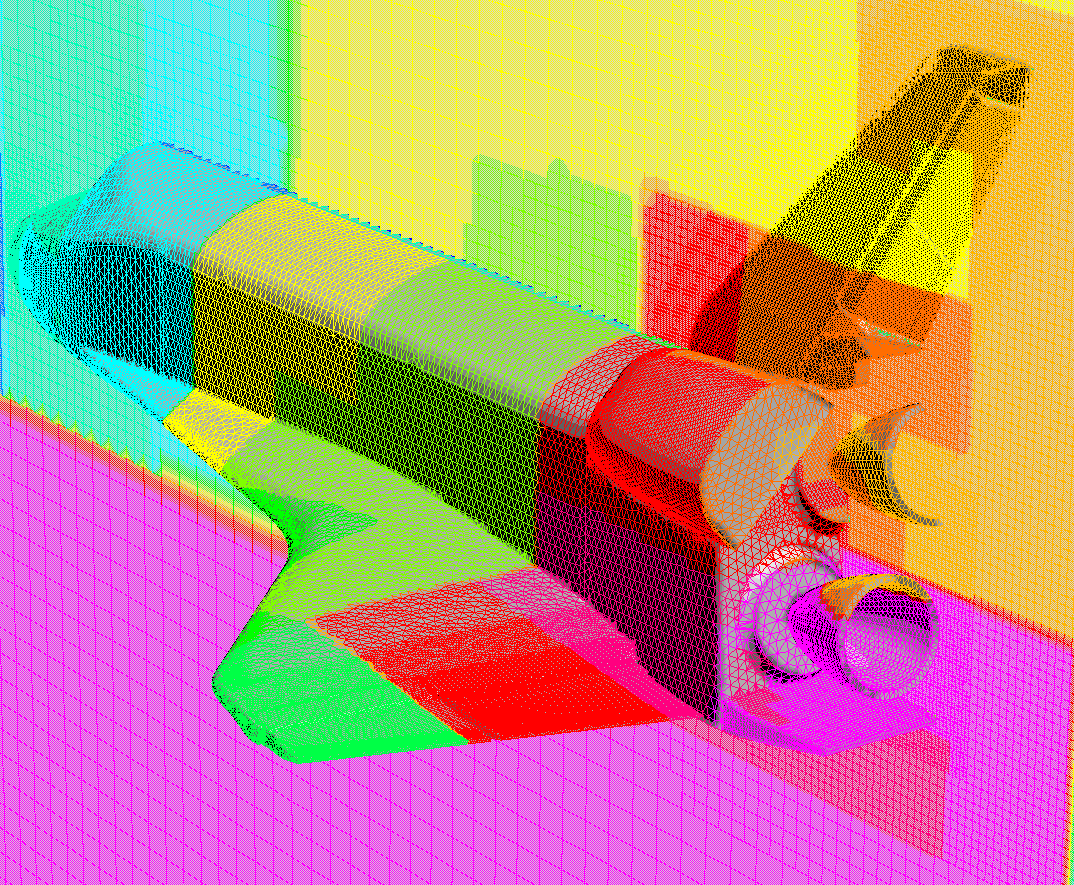
\includegraphics[width=\linewidth]{shuttle16partitions.png}
    \end{column}
    
    \begin{column}{0.4\linewidth}
      Domain decomposition on the exterior of the space
      shuttle. Notice the complicated sub-domain shapes. To create
      these decomposition is a non-trivial problem, and libraries
      should be used. Communication between sub-domains is very
      complex in such situations, and requires significant
      book-keeping. (Caveats about unstructured meshes)
    \end{column}
  \end{columns}  

\end{frame}
%----------------------------------------------------------------

%----------------------------------------------------------------
\begin{frame}{Use Ghost/Skin cellscommunicate between sub-domains}

  Consider the finite-difference approximation to $g=f_{xx}$
  \begin{align*}
    g_i = \frac{f_{i+1}-2 f_{i}+f_{i-1}}{\Delta x^2}
  \end{align*}
  Now let $I$ be the last cell on a sub-domain boundary. Then, we have
  \begin{align*}
    g_I = \frac{f_{I+1}-2 f_{I}+f_{I-1}}{\Delta x^2}
  \end{align*}
  Note we do not know what $f_{I+1}$ is as it is \emph{outside} the
  sub-domain. I.e. it either lies outside the physical boundary or on
  another sub-domain.%
  \vskip0.1in%
  These outside cells are called ``ghost cells''. They are very useful
  for applying boundary conditions and are \emph{essential} for
  synchronization across cores when doing a parallel job.

\end{frame}
%----------------------------------------------------------------

%----------------------------------------------------------------
\begin{frame}{Ghost cells are the layer of cells \emph{outside}
    sub-domain}

  \begin{columns}
    
    \begin{column}{0.6\linewidth}
      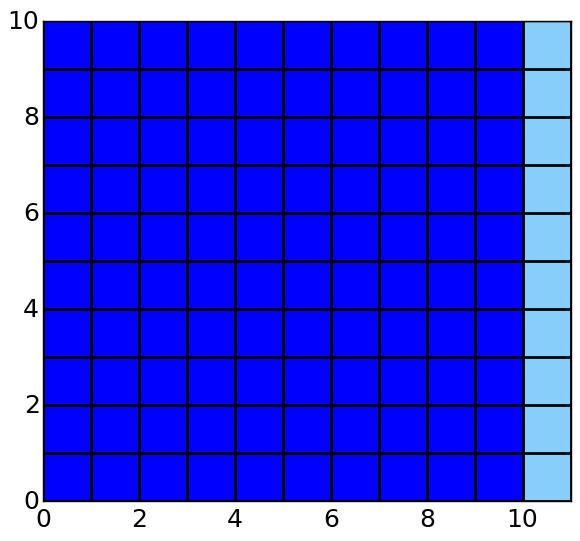
\includegraphics[width=0.9\linewidth]{ghost-cells.png}
    \end{column}
    
    \begin{column}{0.4\linewidth}
      The layer of cells on the right (pale blue) are the \emph{ghost
        cells} for the sub-domain (blue). They lie \emph{outside} the
      sub-domain.
    \end{column}
  \end{columns}

\end{frame}
%----------------------------------------------------------------

%----------------------------------------------------------------
\begin{frame}{Skin cells are layer of cells \emph{inside} sub-domain}

  \begin{columns}
    
    \begin{column}{0.6\linewidth}
      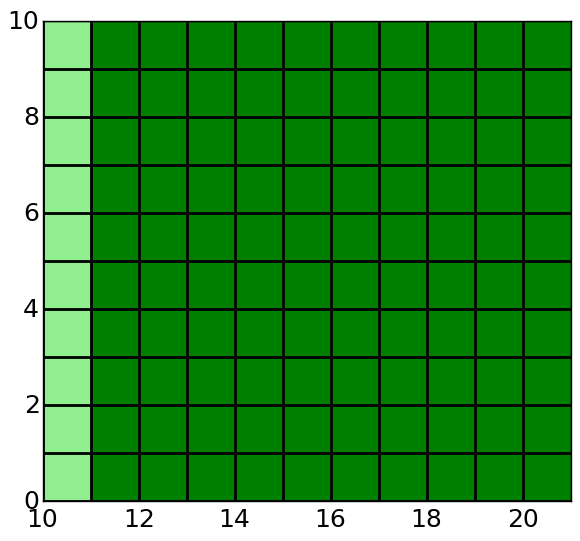
\includegraphics[width=0.9\linewidth]{skin-cells.png}
    \end{column}
    
    \begin{column}{0.4\linewidth}
      The layer of cells on the left (pale green) are the \emph{skin
        cells} for the sub-domain (blue). They lie \emph{inside} the
      sub-domain.
    \end{column}
  \end{columns}  

\end{frame}
%----------------------------------------------------------------

%----------------------------------------------------------------
\begin{frame}{To synchronize copy data from skin-cells to ghost-cells}

  \begin{figure}
    \setkeys{Gin}{width=0.35\linewidth,keepaspectratio}
    \incfig{ghost-cells.png}
    \incfig{skin-cells.png}
    \caption{Before each time-step we must copy data from pale green
      region on right sub-domain into the pale blue region on left
      sub-domain.}
  \end{figure}  

\end{frame}
%----------------------------------------------------------------

%----------------------------------------------------------------
\begin{frame}{Ghost/Skin cell distribution is determined by the
    \emph{stencil}}

  \begin{figure}
    \setkeys{Gin}{width=0.3\linewidth,keepaspectratio}
    \incfig{5point-laplacian.png}
    \incfig{9point-laplacian.pdf}
    \caption{5-point stencil (left) and 9-point stencil (right) for a
      Laplacian in 2D. Note that the 9-point stencil needs corner
      cells. This means that parallel communication must involve
      neighbors which share a \emph{corner} (and not just face
      neighbors). This can significantly complicate communication.}
  \end{figure}

\end{frame}
%----------------------------------------------------------------

%----------------------------------------------------------------
\begin{frame}{For unstructured meshes, things can get \emph{very}
    nasty}

  \begin{columns}
    
    \begin{column}{0.4\linewidth}
      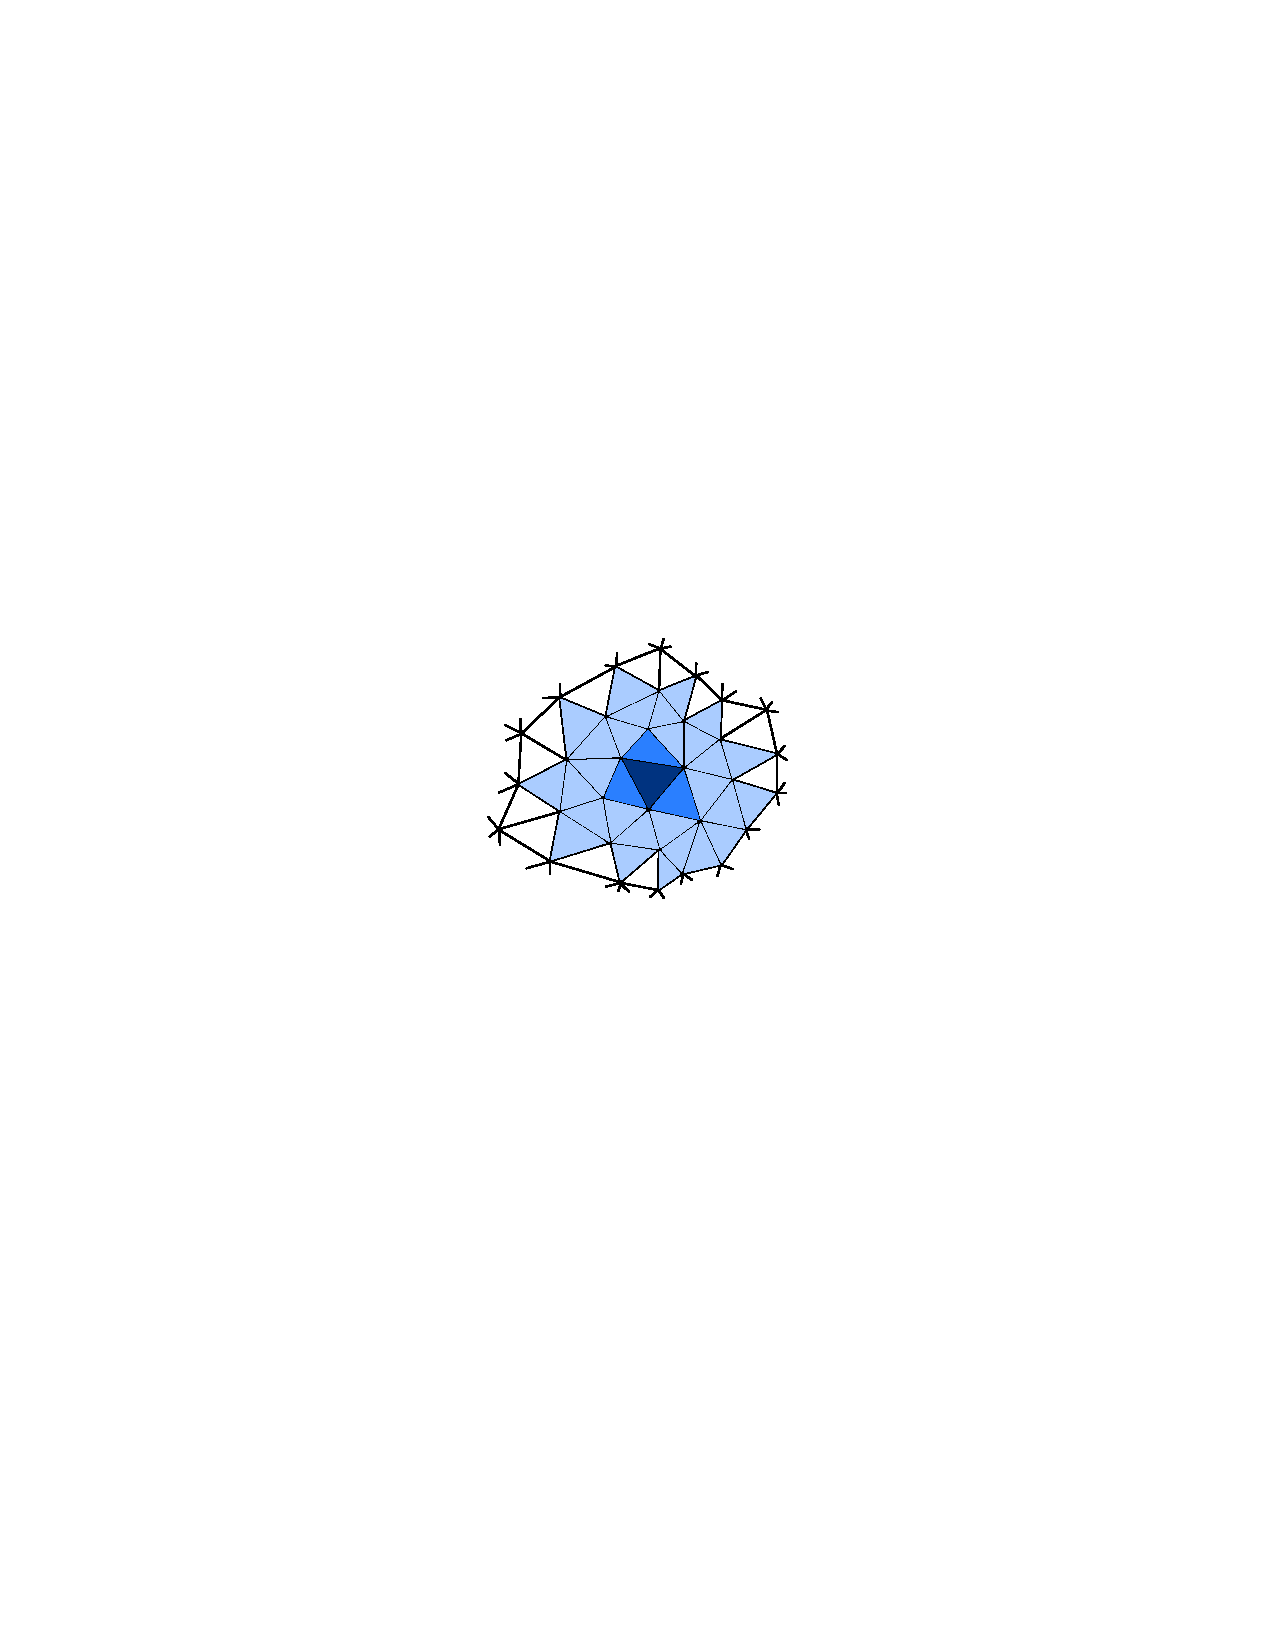
\includegraphics[width=1.0\linewidth]{unstruct-stencil.pdf}
    \end{column}
    
    \begin{column}{0.6\linewidth}
      To update dark blue cell, some scheme would need only face
      neighbors. However, some higher-order methods would need a
      bigger stencil, shown here in pale blue for a third order
      finite-volume scheme. The ghost/skin cell determination and
      parallel communication is very complicated.
    \end{column}
  \end{columns}

\end{frame}
% ----------------------------------------------------------------

%----------------------------------------------------------------
\begin{frame}{Alice and Bob eat lunch}

  {\color{blue} Imagine Alice is in one city, and Bob in another. How
    can we ensure Alice eats lunch \emph{before} Bob?}  \vskip0.1in%
  \mypause%
  Note that we can't rely on clocks, as clocks may not be accurate,
  and not every event (in life as well a computer) has a time-stamp
  associated with it.%
  \vskip0.1in%
  \mypause%
  Obvious solution: Bob \emph{waits} for Alice to call him after she
  eats lunch. Then Bob eats lunch. (Blocking receive)%
  \vskip0.1in%
  \mypause%
  Bob keeps doing his stuff, and every time he gets hungry, he checks
  if Alice left him the \emph{correct} message. If yes, he eat, or
  else he goes back to doing other things. (Non-blocking receive)%
  \vskip0.1in%
  \mypause%
  If Alice never calls, Bob will starve to death.
\end{frame}
% ----------------------------------------------------------------

%----------------------------------------------------------------
\begin{frame}{MPI Communicators, rank and blocking/non-blocking calls}
  \footnotesize%
  \begin{itemize}
  \item Cores can be grouped to form communicators ({\tt
      MPI\_Comm}). When program starts, a global communicator with all
    cores is created for you ({\tt MPI\_COMM\_WORLD}). You can create
    sub-communicators if you want (rarely need to do this).
  \item The rank of a cores is an integer \emph{starting from 0}. Each
    core has a unique rank.
  \item For many communication methods, there are \emph{blocking} and
    \emph{non-blocking} versions.
  \item When you use a \emph{blocking} version of a call, the code waits
    for the operation to be completed.
  \item When you use a \emph{non-blocking} version of a call, the code
    immediately continues, \emph{even if the operation is not
      complete}.
  \item Non-blocking calls can be more efficient, as you can overlap
    communication and computation. However, it can lead to nasty
    bugs. In particular, non-blocking receives are very confusing. You
    \emph{must not} use the ``received'' data before it is actually
    received.
  \item MPI provides means of waiting for a send or receive to
    finish. These must be used to get synchronization correct.
  \end{itemize}
  
\end{frame}
%----------------------------------------------------------------

%----------------------------------------------------------------
\begin{frame}{To send/receive one needs to use {\tt MPI\_Send} and
    {\tt MPI\_Recv}}

  There are two versions of each call
  \begin{itemize}
  \item \emph{Blocking} versions {\tt MPI\_Send} and {\tt MPI\_Recv}.
    The blocking calls will \emph{block} till the send/receive are
    completed.
  \item \emph{Non-blocking} versions {\tt MPI\_Isend} and {\tt
      MPI\_Irecv}.   The non-blocking calls will \emph{return immediately} even if the
    send/receive are not completed yet.
  \end{itemize}
  \mypause%
  \vskip0.1in%
  How to determine if the send/receive are actually completed or not?%
  \vskip0.1in%
  {\color{blue} Each non-blocking class returns to the caller a {\tt
      MPI\_Request} ``token''. This can be used in the {\tt MPI\_Wait}
    method to wait till the operation with that ``token'' is
    completed.}%
  \vskip0.1in%
  Think of this as a ``will call'' system. You buy tickets online and
  print out a receipt at home. Before the show you go to the ``will
  call'' counter with the receipt and pick up your tickets.

\end{frame}
%----------------------------------------------------------------

%----------------------------------------------------------------
\begin{frame}{The anatomy of {\tt MPI\_Send}}

  {\color{blue} {\tt int MPI\_Send(const void $*$buf, int count,
      MPI\_Datatype datatype, int dest, int tag, MPI\_Comm comm)}}
  \begin{itemize}
  \item \myb{{\tt buff}}\ Is the pointer to the array you want to send
  \item \myb{\tt count}\ Is the size of the array you are sending
  \item \myb{\tt datatype}\ Is the type of data you are sending (doubles,
    floats, ...)
  \item \myb{\tt dest}\ Is the rank of the \emph{destination} core you want
    to send the array to
  \item \myb{\tt tag}\ is a unique tag attached to each message (this
    distinguishes multiple message between the same pair of
    communicating cores)
  \item \myb{\tt comm}\ Is the communicator group you are using
  \end{itemize}
  The {\tt MPI\_Recv} signature is analogous. Note that \emph{a send
    must be balanced by a receive or the code will hang!}.

\end{frame}
%----------------------------------------------------------------

%----------------------------------------------------------------
\begin{frame}{With {\tt MPI\_Irecv} call you \emph{must} wait before
    you use the data}
  
  After calling a {\tt MPI\_Irecv} (non-blocking call) you can do
  other things. However, \emph{before} you use the data you are
  expecting, you must wait by calling the {\tt MPI\_Wait} with the
  ``token'' which {\tt MPI\_Irecv} gave you.%
  \vskip0.1in%
  In addition, you must not send any more data before the receive is
  completed. Otherwise terrible things will happen!%
  \vskip0.1in%
  {\color{blue} In short: when you can, use \emph{blocking}
    calls. Reasoning about non-blocking calls is hard and can lead to
    very subtle bugs which may only show up when you run on a large
    machine. Remember Murphy's Law: ``Anything that can go wrong, will
    go wrong''}

\end{frame}
%----------------------------------------------------------------

%----------------------------------------------------------------
\begin{frame}{Summary of distributed programming with MPI}

  \begin{itemize}
  \item The standard pattern of distributed programming is: decompose,
    initialize and then in a loop, do local updates, and then
    communicate ghost/skin cell data.
  \item You only need to know a few methods to write most solvers in
    parallel. {\tt MPI\_Comm\_size}, {\tt MPI\_Comm\_rank}, {\tt
      MPI\_Allreduce}, {\tt MPI\_Send} and {\tt MPI\_Recv} will cover
    90\% of your needs.
  \item You must carefully look at your scheme's stencil to determine
    which of your neighbors you need to send/receive data
    to/from. \emph{Avoid} schemes with more that one or two
    ghost/skin-cells. I.e. don't use a scheme which has a wide
    stencil.
  \end{itemize}

\end{frame}
%----------------------------------------------------------------

\end{document}

% ----------------------------------------------------------------
\begin{frame}{}
\end{frame}
% ----------------------------------------------------------------

\begin{columns}
  
  \begin{column}{0.6\linewidth}
  \end{column}
  
  \begin{column}{0.4\linewidth}
    \includegraphics[width=\linewidth]{fig/Kinsey_2011_Pfus_vs_T.pdf}
  \end{column}
\end{columns}

% ----------------------------------------------------------------

\begin{columns}

  \begin{column}{0.4\linewidth}
    \includegraphics[width=\linewidth]{fig/Kinsey_2011_Pfus_vs_T.pdf}
  \end{column}
  
  \begin{column}{0.6\linewidth}
  \end{column}
  
\end{columns}
